\section{The support geometry is uninformative, so the step is a fixed curve in $K$}\label{sec:finding1}

PARA's step is meant to adapt to the support set: a support set that disagrees with the text should earn a larger step.
On all six datasets, however, $\eta(S)$ is almost entirely determined by the number of shots.
Pooled over datasets and prompt sets, its mean is $0.328$, $0.603$ and $0.798$ at $K = 1$, $4$ and $16$ (Figure~\ref{fig:eta_vs_K}).
The per-dataset means span only $0.316$ to $0.353$, $0.587$ to $0.610$ and $0.790$ to $0.802$,
even though the datasets range from 2 to 11 classes and from near-chance to fairly strong zero-shot anchors.
Across the 10 support draws of a setting, the standard deviation of $\eta(S)$ never exceeds $0.011$.
This section explains why, and shows that a step depending on $K$ alone does at least as well.

\begin{figure}[t]
  \centering
  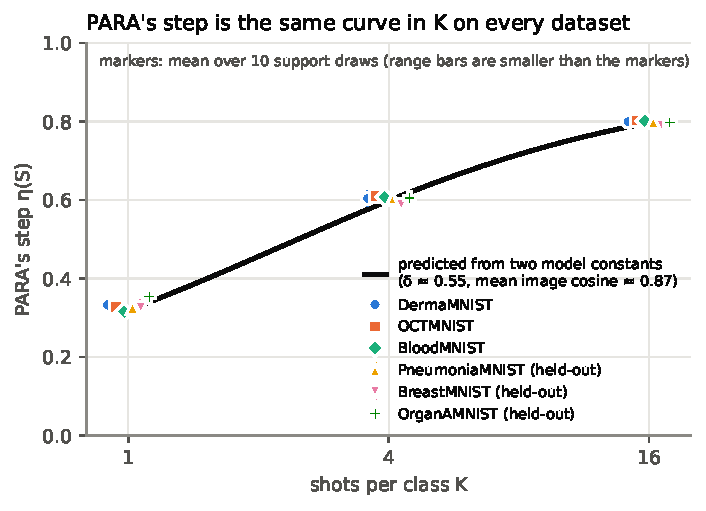
\includegraphics[width=0.62\linewidth]{F1_para_eta_vs_K}
  \caption{PARA's step $\eta(S)$ against shots per class, mean over 10 support draws for each dataset
  (draw-to-draw ranges are smaller than the markers).
  The curve is the prediction of Eq.~\eqref{eq:pred} from two constants of the frozen model,
  $\bar\delta = 0.550$ and the pooled image cosine $0.867$.}
  \label{fig:eta_vs_K}
\end{figure}

\paragraph{The discrepancy $\delta_c$ does not depend on the class.}
Figure~\ref{fig:geometry} (top left) compares, for $K = 16$ and one support draw, each class's discrepancy to its own text
with its discrepancy to the other classes' text.
On five datasets the two differ by only $0.004$ to $0.018$; OrganAMNIST shows the largest gap
($0.604$ against $0.647$).
The support images of a class are closest to their own class text for only one or two classes per dataset
(three of eleven on OrganAMNIST).
In BiomedCLIP's frozen space, image and text embeddings occupy separate regions, the modality gap described by \citet{liang2022mind},
so $\delta_c$ mostly measures the distance between the two modalities, which is the same for every class.
Averaged over the six datasets, the own-text discrepancy is $\bar\delta = 0.550$.

\paragraph{The agreement $\phi_c$ does not depend on the class either.}
Sixteen images of one class give almost the same $\phi_c$ as sixteen random images drawn across classes
(Figure~\ref{fig:geometry}, bottom left): the two differ by at most $1.3\%$ on five datasets and by $16\%$ on OrganAMNIST.
The reason is that the frozen image embeddings lie in a narrow cone.
The mean cosine between two support images is $0.839$ to $0.962$ on five datasets, whether or not the images share a class,
and $0.671$ for different-class pairs on OrganAMNIST.
Because the $u_i$ have unit length, $\phi_c$ is an exact function of that cosine:
\begin{equation}
  \phi_c = \frac{1}{n_c} \Big\lVert \sum_{i \in S_c} u_i \Big\rVert^2 = 1 + (n_c - 1)\,\bar c_c,
  \label{eq:phi}
\end{equation}
where $\bar c_c$ is the mean pairwise cosine within class $c$.
When every pair of images has a cosine near 0.9, $\phi_c$ is close to its maximum $n_c = K$ for any class, and for a random set of images as well.

\begin{figure}[t]
  \centering
  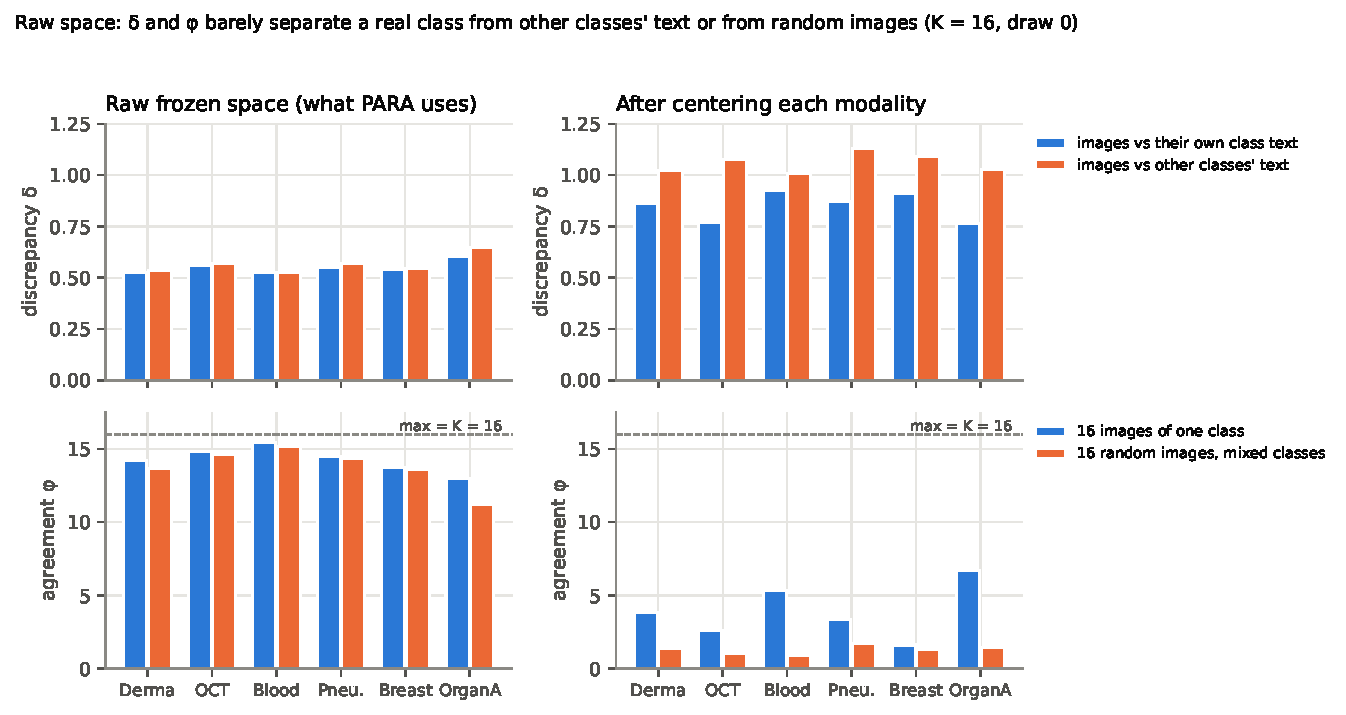
\includegraphics[width=\linewidth]{F2_geometry_check}
  \caption{Support geometry for $K = 16$, one draw per dataset.
  Top: discrepancy of each class's images to their own text and to the other classes' text.
  Bottom: agreement $\phi$ of 16 images of one class against 16 random images from mixed classes.
  Left: the raw frozen space that PARA uses. Right: after subtracting each modality's mean.}
  \label{fig:geometry}
\end{figure}

\paragraph{Two constants predict the step.}
If every class has $\delta_c \approx \bar\delta$ and $\bar c_c \approx \bar c$, Eqs.~\eqref{eq:eta} and~\eqref{eq:phi} give
\begin{equation}
  \eta(K) \approx \lambda\,\frac{a(K)}{1 + a(K)}, \qquad a(K) = \bar\delta\,\big(1 + (K - 1)\,\bar c\big).
  \label{eq:pred}
\end{equation}
With $\bar\delta = 0.550$ and the mean same-class cosine $\bar c = 0.886$, Eq.~\eqref{eq:pred} predicts
$0.319$, $0.601$ and $0.798$ at $K = 1$, $4$ and $16$, against the measured $0.328$, $0.603$ and $0.798$.
Using the cosine pooled over same- and different-class pairs ($0.867$, the curve in Figure~\ref{fig:eta_vs_K}) changes the prediction by about $0.003$ at most,
which is itself a symptom: the class structure that $\phi_c$ is meant to detect hardly registers.
At $K = 1$, $\phi_c = 1$ exactly, so the step there depends on $\delta_c$ alone.

OrganAMNIST deserves a note, because it is the one dataset where the geometry does carry some class signal
(the largest $\delta$ gap and a $16\%$ higher $\phi$ for real classes).
Its step still lies on the same curve ($0.353$, $0.605$ and $0.797$),
because the signal is small relative to the shared offset $\bar\delta$ and the near-saturated $\phi_c$.

\paragraph{The step does not track the best step.}
Within a setting, the small draw-to-draw variation of $\eta(S)$ is not informative either.
Its Spearman correlation with the best $\eta$ for each draw (chosen on the test set, after removing each setting's mean)
is $-0.12$ ($p = 0.04$): weakly negative, and of no practical use.

\paragraph{A step that depends on $K$ alone does at least as well.}
If the geometry adds nothing, the shot-only schedule $\eta_K = \lambda K / (1 + K)$ ($0.45$, $0.72$ and $0.85$) should match PARA.
It does better.
On the design datasets it raises mean BAcc by $2.65$ points, wins 150 of 179 non-tied draws,
and is significantly better in 13 of 18 settings (8 after Holm's correction) and significantly worse in none.
On the held-out datasets the gain is $0.82$ points (3 of 12 settings better, none worse).
All of that gain comes from OrganAMNIST ($3.27$ points, 3 of 3 settings).
On the two binary held-out datasets the two steps give identical predictions on every draw,
for a reason we explain in Section~\ref{sec:finding2}.

\paragraph{Centering makes the geometry informative but does not give a better step.}
Subtracting each modality's mean embedding before computing Eq.~\eqref{eq:eta} restores class information
(Figure~\ref{fig:geometry}, right): real-class agreement rises to $1.62$ to $6.73$ against $0.94$ to $1.74$ for random sets,
and the own-text discrepancy ($0.764$ to $0.926$) falls below the other-text discrepancy ($1.010$ to $1.130$) on all six datasets.
The resulting step is still not better: averaged over the design datasets it gives $55.79$ BAcc against $57.54$ for PARA,
and it is worse than PARA on 5 of 6 datasets.
Knowing how coherent a class looks in the frozen space is not what the step needs;
Section~\ref{sec:finding3} argues that what matters is how reliable the anchor is relative to the trained branch.
